\documentclass[sigconf]{acmart}
\AtBeginDocument{%
  \providecommand\BibTeX{{%
    \normalfont B\kern-0.5em{\scshape i\kern-0.25em b}\kern-0.8em\TeX}}}

\settopmatter{printacmref=false}
\setcopyright{none}
\renewcommand\footnotetextcopyrightpermission[1]{}
\pagestyle{plain}

\setcopyright{none}
\makeatletter
\renewcommand\@formatdoi[1]{\ignorespaces}
\usepackage{geometry}
\usepackage{fancyhdr}
\usepackage{pdfpages}
\usepackage{xparse}
\usepackage{kantlipsum}
\NewDocumentCommand\headerspdf{ O {pages=-} m }{% [options for include pdf]{filename.pdf}
  \includepdf[%
    #1,
    pagecommand={\thispagestyle{plain}},
    scale=.7,
    ]{#2}}
\NewDocumentCommand\secpdf{somO{1}m}{% [short title]{section title}[page specification]{filename.pdf} --- possibly starred
  \clearpage
  \thispagestyle{plain}%
  \includepdf[%
    pages=#4,
    pagecommand={%
      \IfBooleanTF{#1}{%
        \section*{#3}}{%
        \IfNoValueTF{#2}{%
          \section{#3}}{%
          \section[#2]{#3}}}},
    scale=.65,
    ]%
    {#5}}
\makeatother
\graphicspath{{./images/}} 

\begin{document}

\title{CineGPT: Generative A.I. In Screenwriting}


\author{Ryan Harding}
\email{ry287616@ucf.edu}
\affiliation{%
  \institution{University of Central Florida}
  \city{Orlando}
  \state{Florida}
  \country{USA}
  \postcode{32816}
}

\begin{abstract}
The use of A.I. in Screenplay has been a controversial topic in the film industry, with arguments for it as an escape from barriers of entry and arguments against dealing with ethical and authorship issues. To determine both the potential uses and limitations, as well as to validate and test concerns with the technology, I created an original story treatment and screenplay and ran through several generative A.I. experiments to test the potential of ChatGPT in these fields. I generated A.I. screenplays from a treatment and compared against my original work, and used A.I. to critique and analyze the resulting scripts.
\end{abstract}

\maketitle

\textbf{Artifact and Resource Repository:}\\
https://github.com/rharding8/CineGPT

\section{Introduction}
\indent As someone invested both in technology and filmmaking, the use of A.I. in filmmaking is one that gives me pause. Some screenwriters noted fears over A.I. replacing them, or losing valuable credit and residuals due to the use of A.I., during the 2023 Writer's Guild of America Strikes \cite{Kinder_2024}. Other screenwriters instead have expressed belief in A.I. being unable to eclipse human work, supporting its use in brainstorming, storyboarding, and revision. Even some of these writers, however, have noted these uses can encroach on entry-level writer positions in television \cite{Deese_2024}. Because of this, I decided to research within Topic 14 (Natural Language to Video Storyboarding), to determine where A.I. falls short in filmmaking, where it succeeds, and how to limit its role in replacing human creativity while enhancing its role in aiding it.
\section{Related Work}
\indent Many studies have gone into the technical and creative sides of this issue, exploring how screenplay analysis and generation and storyboard generation work computationally, the concerns associated with such, and the creative implications. A study by Sabyasachee Baruah and Shrikanth Narayanan went into detail about the limitations and concerns of character coreference resolution, a subset of named-entity-recognition (NER) related to characters within the screenplay. Baruah and Narayanan discussed how screenplay length often exceeds the limits of traditional transformers, requiring a new set of approaches using BERT models as well as Bidirectional RNNs to parse and resolve references in a screenplay. They also noted concerns about non-linear stories and characters being referred to as a plural (E.g. "Kids"), which I've taken into account to make sure my work can be analyzed properly \cite{baruah-narayanan-2023-character}.\\
\indent NER concerns were also noted by Kyle Jorgenson and Haohong and Mea Wang from the University of Calgary, who conducted a study and experiment to create a simple script-to-film pipeline using A.I. to generate an animated film from a human-written screenplay. They believed such a tool could remove barriers of entry to people looking to make films, allowing writers to take control into their own hands and produce their vision without any other technical skill required \cite{10074526}. Their program, using script coverage and NER through transformers, takes advantage of pre-made assets and a Unity environment to allow a writer to automatically generate environments and place characters within it. They can even line-up recorded voices with dialogue in the script to automatically voice the film \cite{10074526}. The program essentially takes the role of the crew, while the writer becomes director and producer of the film. However, even this experiment still required considerable user-input and decision-making, proving A.I. analysis and placement was still imperfect \cite{10074526}.\\
\indent A more creatively-minded study into A.I. for script generation, rather than just analysis and visual generation, was conducted by Susan Cake, who explored using ChatGPT and other models as both a collaborator and primary writer. Cake noted that such tools had already become commonplace in analytics and post-production tasks, risking infringing on jobs in those fields, and could raise concern for writers as well \cite{Cake20012025}. Cake explored risks such as the homogeneity of A.I.-produced scripts, copyright infringement concerns about scripts used to train Large Language Models (LLMs), and legal concerns around guidelines in different nations around media involving sensitive subjects \cite{Cake20012025}. The latter being especially relevant given recent controversy around DeepSeek and censorship around subjects such as Tiananmen Square \cite{Lu_2025}.\\
\indent Cake was also concerned about cultural prejudices, especially from a non-American perspective she found ChatGPT to typically lean into American culture and screenwriting conventions even when given Australian stories \cite{Cake20012025}. She ultimately found that results were not up to par with human work, with ChatGPT 3.5 creating cliched dialogue and generic plotlines, sometimes lacking basic cause-and-effect. True to her concerns, she found the results could contain copyrighted material and harmful stereotypes and often leaned towards generic "happy endings" \cite{Cake20012025}. Cake also noted that ChatGPT was better at critiquing work than generating it, but that critiques of A.I.-generated material were almost universally positive and failed to point out obvious flaws, being inconsistent with the quality of the material \cite{Cake20012025}. Because of this I decided to keep an eye out for these issues in my experiment.
\section{Methodology}
\subsection{The First Act}
\begin{figure}[!hbt]
    \centering
    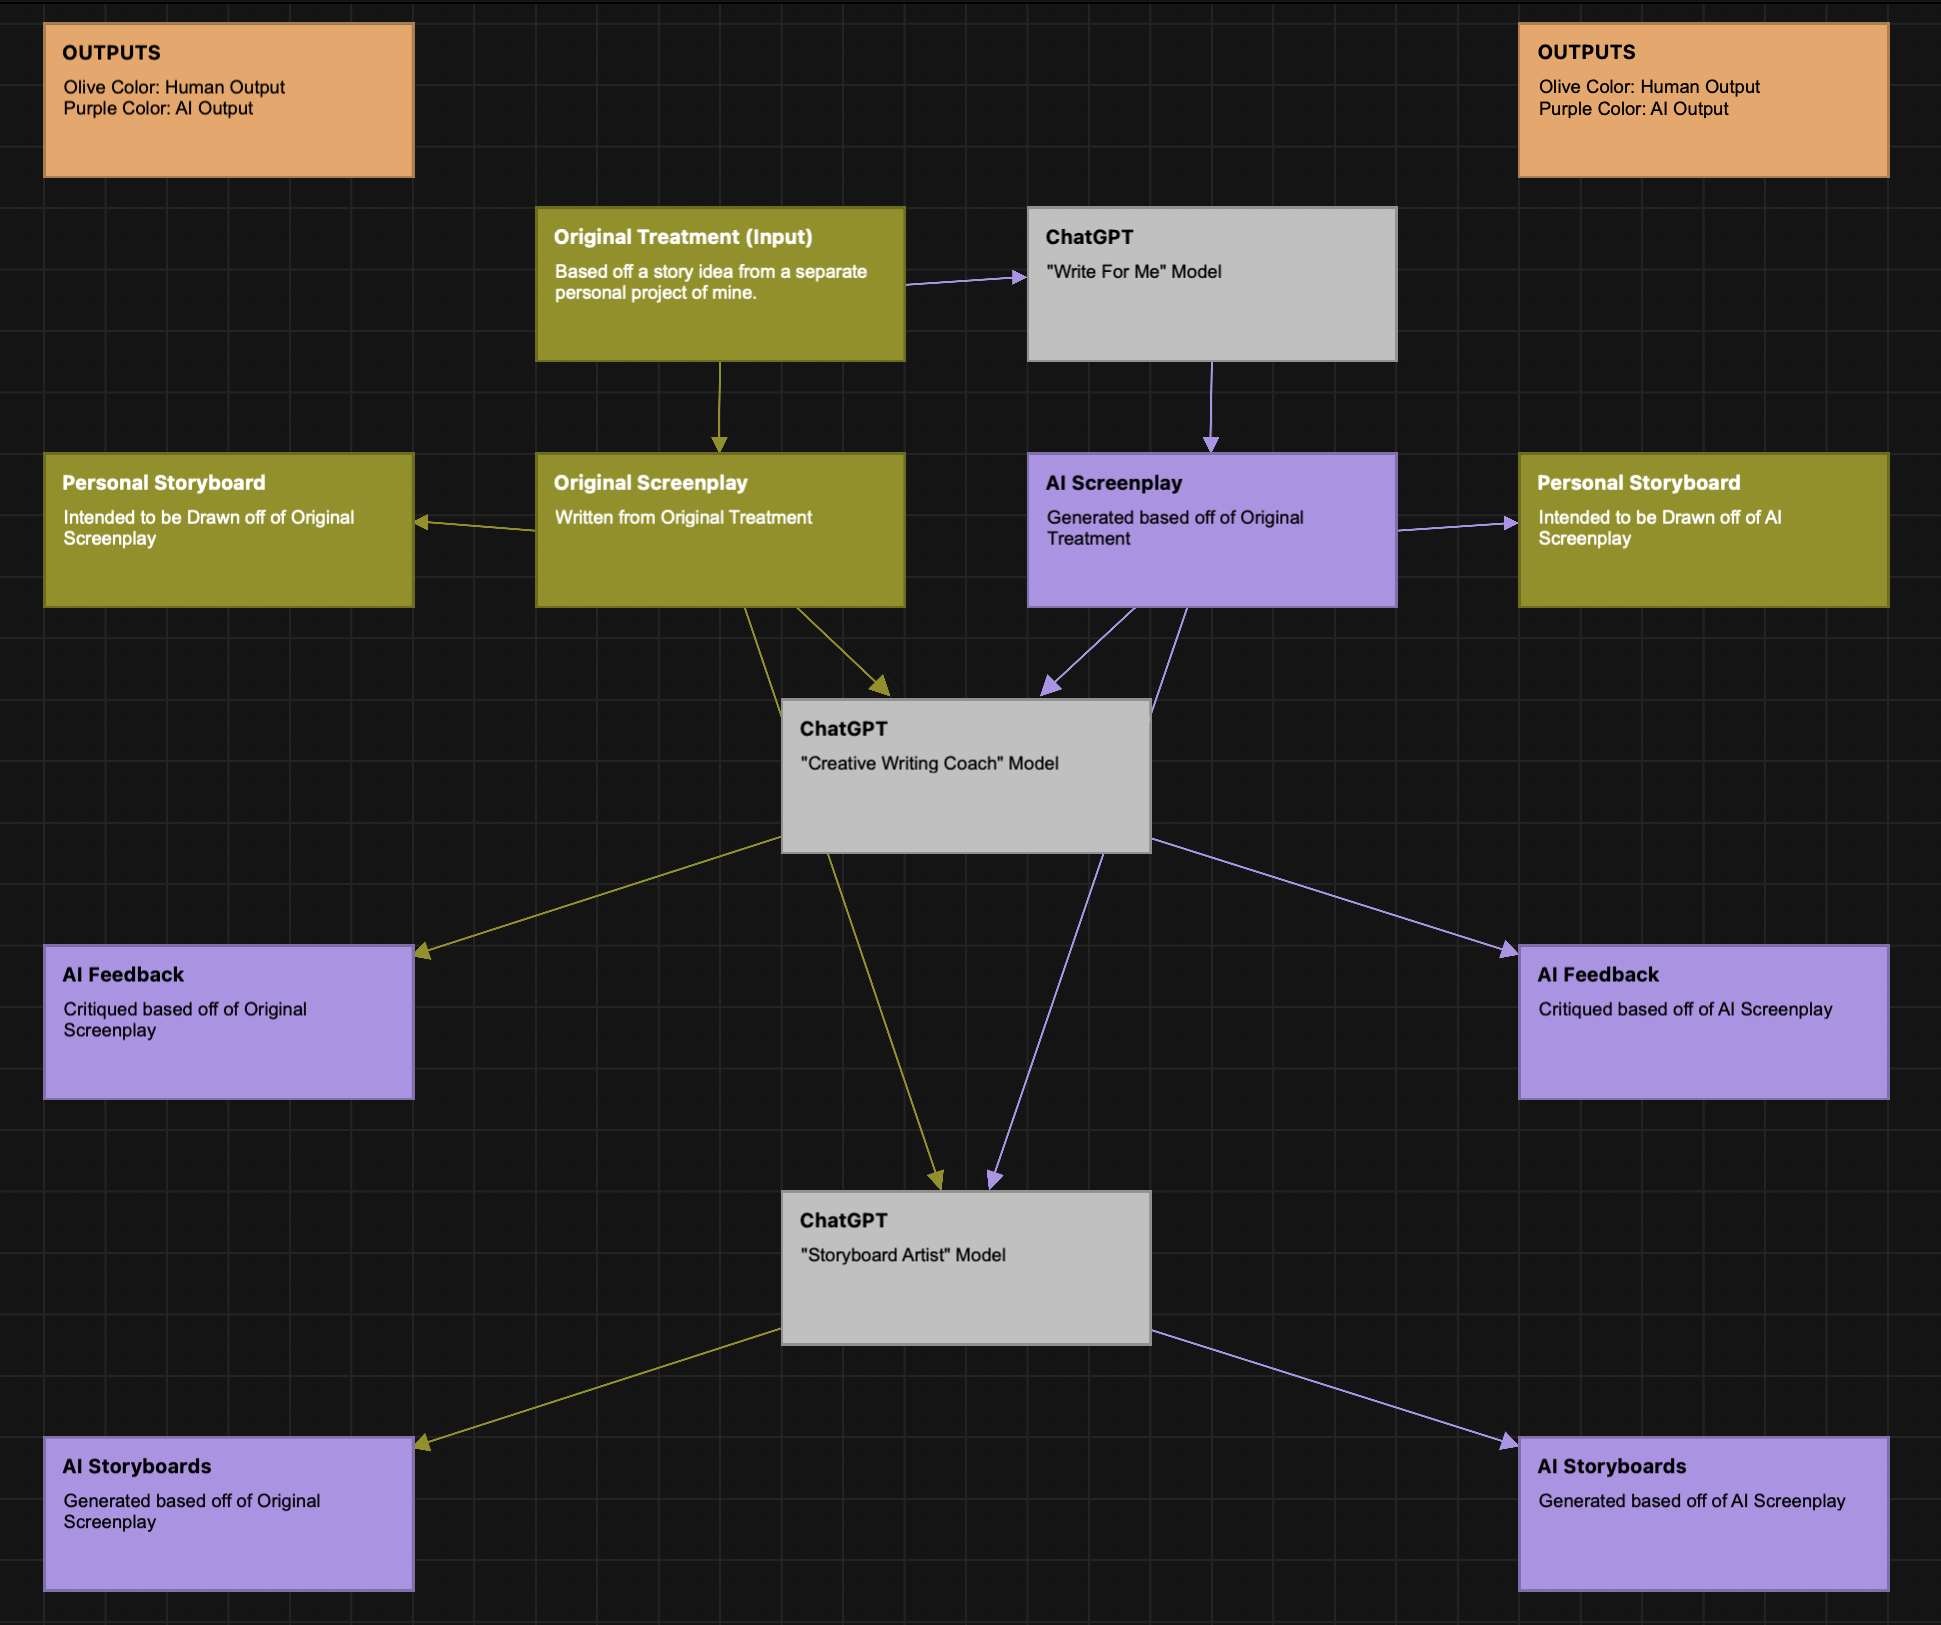
\includegraphics[width=0.8\linewidth]{images/ScrappedPipeline.png}
    \caption{The original intended pipeline for this project, before the screenplay generation experiment was expanded and the storyboard generation experiment was truncated}
    \label{fig:scrapped-pipeline}
\end{figure}
\indent The experiment began by coming up with an initial story idea. I took a piece of an original screenplay I'd already been working on, the opening montage, and used it as a seed to create a short film story. I focused on writing a heavily detailed treatment. Then I got to work on the actual screenplay based on the treatment. It was during this time when I also did most of my wider research for the project, as writing the script itself was the longest portion of the project. I initially sought to write at least one draft of the screenplay \textit{before} any NLP usage was involved, however I decided to initially focus on a first act for the purposes of the milestone earlier this semester. I took that complete first act through the pipeline in Figure 1, minus the storyboard generation.\\
\indent I started by giving ChatGPT, using the "Write For Me" model, the first act of my treatment and instructed it to write a 5-8 page first act screenplay based on it. I then made hand annotations as notes on the screenplay, as well as similar notes on my original screenplay. Finally, I used OpenAI's "Creative Writing Coach" model in ChatGPT to give AI-Generated Notes on both screenplays.
\subsection{Milestone Results and Adjustments}
\indent I started with a wide range of expectations for the A.I. screenplay, going from an incoherent mess to human quality. I was surprised to see the generated first act was coherent, but only by virtue of following the treatment nearly verbatim. Despite entering a prompt asking for a 5-8 page act, the resulting script was only 3 pages, one more than my treatment. For the most part, the A.I. script just put the treatment into screenplay format, expanded a few lines of dialogue, and added brief moments of imagery. One such moment actually impressed me enough to make note of it for making an image I hadn't thought of, which can be found in Figure 2 \cite{chatgpt}.\\
\begin{figure}[!hbt]
    \centering
    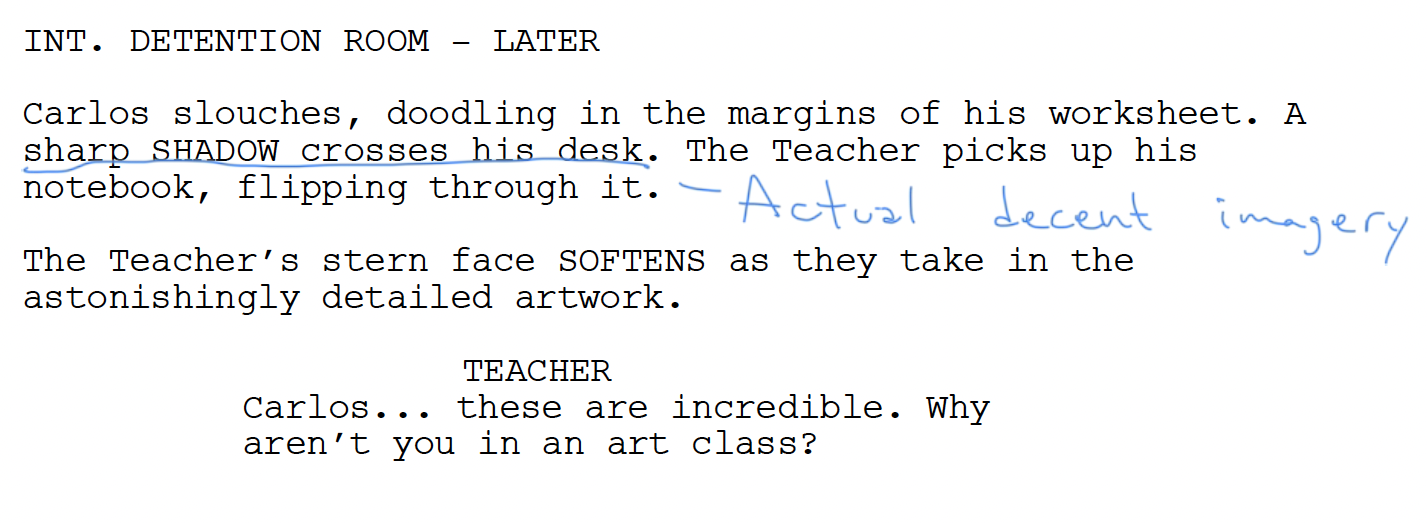
\includegraphics[width=0.8\linewidth]{images/AIA1Imagery.png}
    \caption{A decent use of imagery generated by the first act of the first A.I. script}
    \label{fig:a1-imagery}
\end{figure}
\indent However, the barebones nature of it made it more of an extractive translation than an abstractive expansion. It also made key mistakes in formatting such as using capitalization across the script at random, not just for character names \cite{chatgpt}. And the changes it did make to the characters or narrative were either confusing, cliched, or actively undermining the intent behind the story.\\
\indent For example, Carlos is explicitly defined as arrogant and womanizing in my treatment, leading to a moment where he defends a woman but also hits on her. In the AI screenplay, his tone is not only changed to be harmlessly playful, but his comment is entirely one of support \cite{chatgpt}. The two examples can be seen below, along with my note about Carlos being portrayed as "too nice".\\
\begin{figure}[!hbt]
    \centering
    \begin{minipage}{0.2\textwidth}
        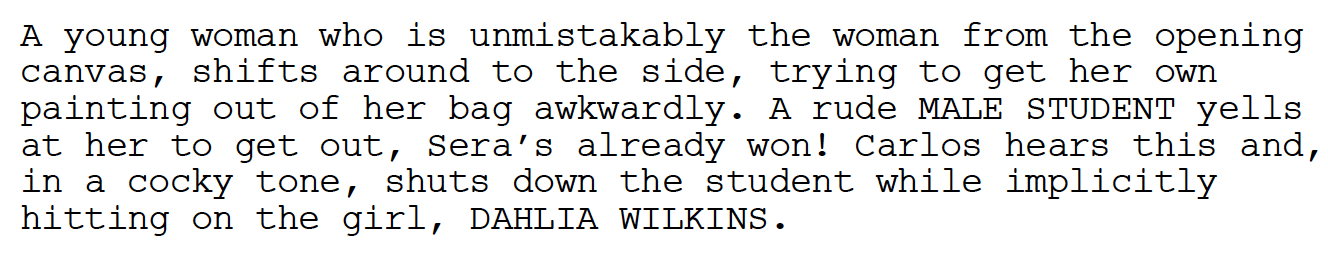
\includegraphics[width=1.0\linewidth]{OGTreatment.png}
        \caption{Original Treatment Description}
        \label{fig:treatment-excerpt}
    \end{minipage}\hfill
    \begin{minipage}{0.2\textwidth}
        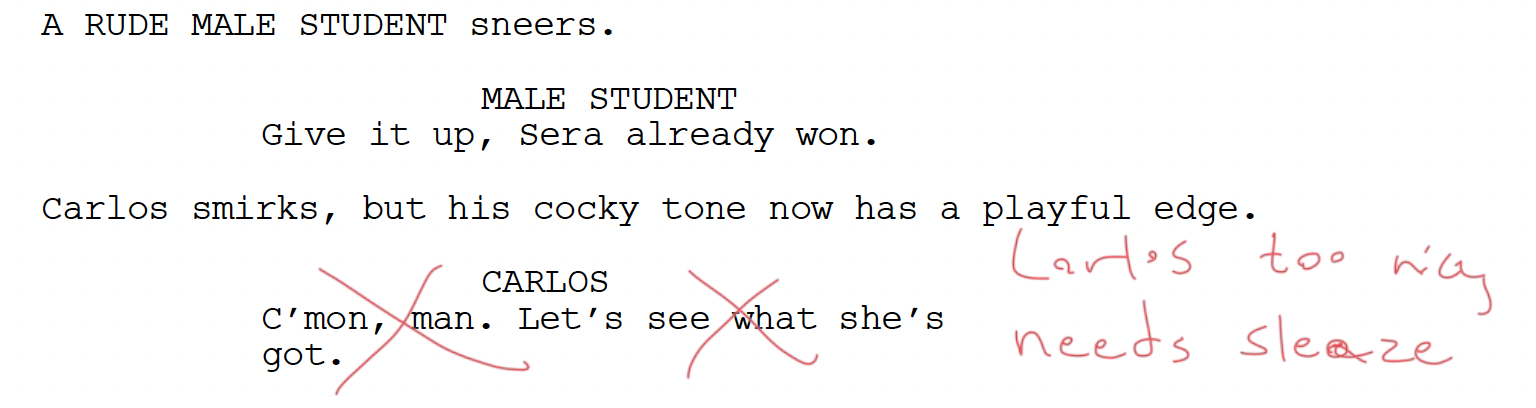
\includegraphics[width=1.0\linewidth]{BadAI.png}
        \caption{Sanitized A.I. Script Interpretation}
        \label{fig:ai-excerpt}
    \end{minipage}
\end{figure}\\
The A.I. first act made no reference to Carlos being a womanizer at all. This overt sanitization felt like the LLM wanting to avoid any sort of prejudice or bias, without recognizing that characters being flawed can be intentional.\\
\indent I had also tested the ability of A.I. to critique and give notes on my own first act, which I had made several critiques and notes on myself. When the "Creative Writing Coach" was tested on my own first act, it gave me valuable feedback including pacing issues, inconsistencies, and how I could improve the commentary of the script \cite{chatgpt}. However, not only did it miss some obvious problems with my first act, including logistical issues of realism, but it too fell prey to the LLM's attempt to avert bias and prejudice by sanitizing some characters. I refer to this criticism of Dahlia's portrayal:
\begin{quote}
    Maybe have her arrive in a different way—she doesn’t just rush in breathless but makes an entrance that asserts her presence in a powerful way \cite{chatgpt}.
\end{quote}
This ignores that Dahlia is set up as struggling a bit, yet proving herself fierce nonetheless. The A.I. suggestion wasn't concerned with staying true to the character or her arc, but rather trying as hard as possible to prove itself unbiased.\\
\indent Finally, I had set ChatGPT to critique the A.I.-generated first act. Consistent with Cake's observations, the resulting critique was almost universally positive, giving the LLM-generation more credit than it deserved and identifying character motivation and detail completely absent from the script itself.\\
\indent At that point I decided to make some adjustments to my process moving forwards:
\begin{enumerate}
    \item In addition to continuing the existing generated screenplays, I would also do a second A.I. screenplay from scratch once the script was finalized. My theory was that having a complete treatment given for a complete script could give more context to character arcs and potentially ease the bias issues I noted.
    \item I would add yet a fourth screenplay to the pipeline by simplifying my treatment down to a two-page treatment, and set ChatGPT to create a screenplay from that as well. My theory being that less railroading and information might give the model more flexibility.
    \item Shortly thereafter, due to the expansion of the screenplay generation experiments, time constraints, and early personal storyboard experiments not being useful due to the lack of a proper talented storyboard artist, I decided to drop the storyboard generation portion of the research. That deserves its own experiments and study, as well as a proper baseline with genuine storyboards that I couldn't guarantee in the duration of this project.
\end{enumerate}
\subsection{The Complete Pipeline}
\begin{figure}[!hbt]
    \centering
    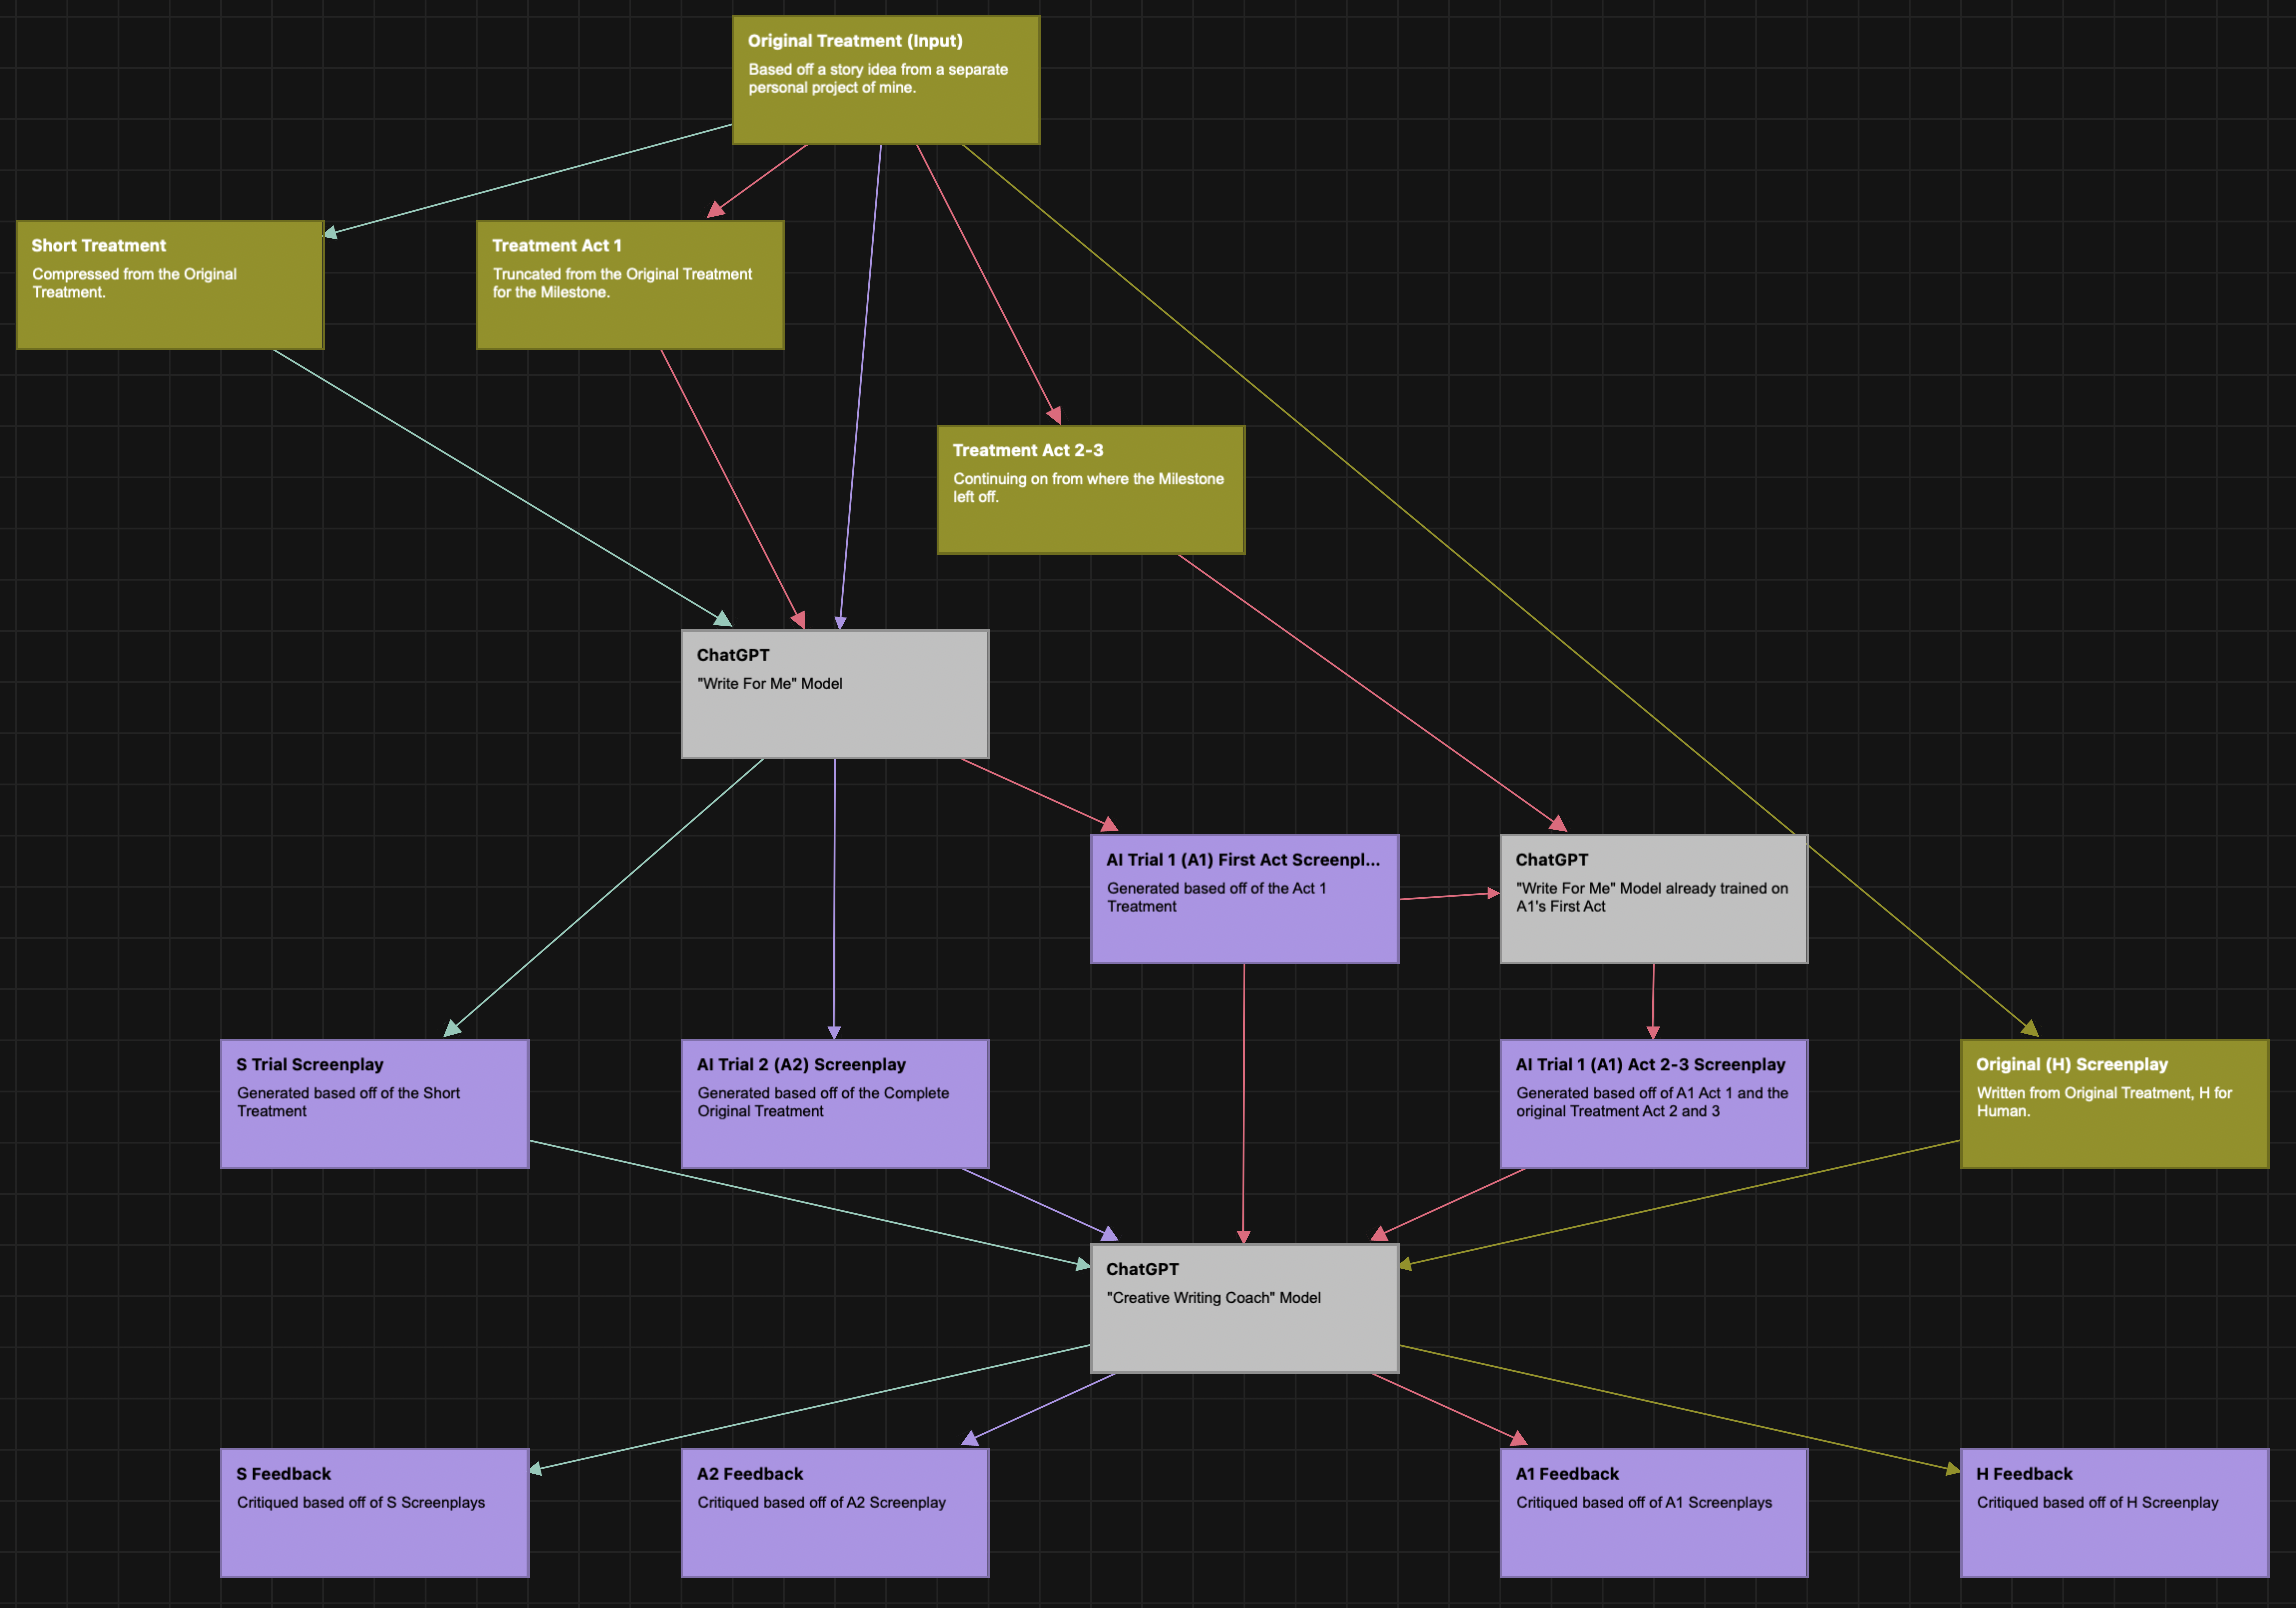
\includegraphics[width=0.8\linewidth]{images/FinalPipeline.png}
    \caption{The final pipeline for this project. Each line color traces a different variation [H, S, A1, A2] of the script.}
    \label{fig:final-pipeline}
\end{figure}
\indent The above is the more complex, comprehensive process I ended up using once the milestone passed. I split my workflow into four separate screenplay projects:
\begin{description}
    \item[H] The 'H' screenplay, or "Human" screenplay, was my own script that I worked on almost all semester long, building off of my original treatment.
    \item[A1] The 'A1' screenplay, or "A.I. Trial 1" screenplay, was the continuation of the screenplay that ChatGPT started back in February. I fed the model both its own Act 1 script and my treatment for Act 2 and 3 to get a consistent result.
    \item[A2] The 'A2' screenplay, or "A.I. Trial 2" screenplay, was a from-scratch screenplay that ChatGPT built off of my complete treatment.
    \item[S] The 'S' screenplay, or "Short Treatment" screenplay, was a screenplay that ChatGPT built off of a much-truncated and compressed version of my treatment.
\end{description}

Once these screenplays were complete, I followed the same process for each, making my own notes as well as feeding them back into the "Creative Writing Coach" model for feedback, and this time receiving quantitative measurements defined by the model based on the metrics I set out for it. All screenplays, treatments, as well as complete conversation histories are found in the Github Repository.

\section{Evaluation and Results}
\subsection{Metrics}
\indent Early on in the project I knew I wanted to judge the screenplays on coherence, pacing, and imagery. For the A.I.-generated critiques, the model defines how to measure these values. For my own human evaluation I decided to lay out a simple points system as follows:
\begin{description}
    \item[Coherency] For coherency, I start reading one of the screenplays with 10 points of coherency, and mark off one point for every break in logic or character. Below 5 points I would deem in need of significant editing, below 0 being a mess.
    \item[Pacing] Similarly, for pacing I start out at 10 points and mark off one for every instance where the story feels noticeably rushed or compressed.
    \item[Imagery] For imagery, I start off at 0 and add a point for every standout image or piece of dialogue I find. Above 5 is good, but 8-10 is where I'd like to be at for a 20+ page screenplay.
\end{description}
In terms of measuring the critiques generated by the A.I., I decided to judge on accuracy and constructiveness:
\begin{description}
    \item[Accuracy] For Accuracy, I follow the same pattern as Coherency and Pacing and subtract points for every problem, only from 5 instead of 10. In this case a problem being the critique extrapolating something clearly not there, embellishing one of the A.I. screenplays, or claiming a flaw as a positive.
    \item[Constructiveness] Much like imagery, this is an additive metric. Every actionable suggestion for improvement on a screenplay is a point, with 5 being a positive result.
\end{description}
\subsection{Human Evaluation}
\begin{description}
    \item[A1] A.I. Trial 1
    \begin{figure}[!hbt]
            \centering
            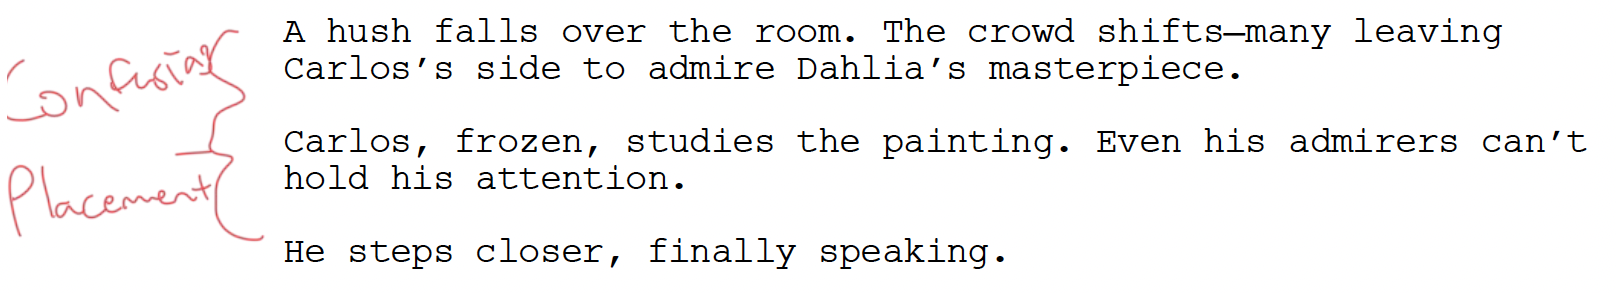
\includegraphics[width=0.8\linewidth]{images/ConfusingPlacement.png}
            \caption{A moment where the logical placement of people in a scene feels completely off in the A.I. generated script}
            \label{fig:a1-confusing}
        \end{figure}
    \begin{description}
        \item[Coherency] was a weak spot with A1. The first act that I had already studied by the milestone contained 5 breaks in coherency alone, including deviations-of-character such as Carlos being sanitized and less of a bully, wrong location placements, and even the staging of an early scene being off, which can be seen in Figure 6.
        Results actually worsened in the second and third act, with multiple out-of-character decisions and dialogue, unclear time jumps, incorrect formatting and terminology leading to a confusing screenplay, and one particularly odd moment of narration being added to the screenplay despite otherwise completely lacking it, as can be seen in Figure 7. Acts 2 and 3 featured 9 breaks in coherency, rendering my score for this section at a $-4/10$ overall.
        \begin{figure}[!hbt]
            \centering
            
\includegraphics[width=0.8\linewidth]{images/Narration.png}
            \caption{A sudden change in tone occurs when the A.I. decides the script suddenly has voiceover}
            \label{fig:a1-narrator}
        \end{figure}
        \item[Pacing] and length in general wound up being a recurring problem across all the A.I. scripts. Despite constantly prompting for a 20-30 page screenplay, none of the A.I. screenplays go over 10 pages long, and most of them hang around the exact same length as the treatment I fed them. As such, pacing is practically non-existent across these scripts.\\
        A1 consistently rushed past major, important scenes, while also giving unnecessary time to unimportant ones. I made note of 9 times I felt the pacing was rushed in unnecessary montages or scenes lacking detail or breathing room, rendering my score a $1/10$.
        \item[Imagery] actually wasn't terrible here. Dialogue was often cliche and never really stood out, but a few visual images did. I will once again highlight Figure 2 as decent image, though it was the only one that stuck with me enough to give it a single point.
    \end{description}
    \item[A2] A.I. Trial 2
    \begin{figure}[!hbt]
            \centering
            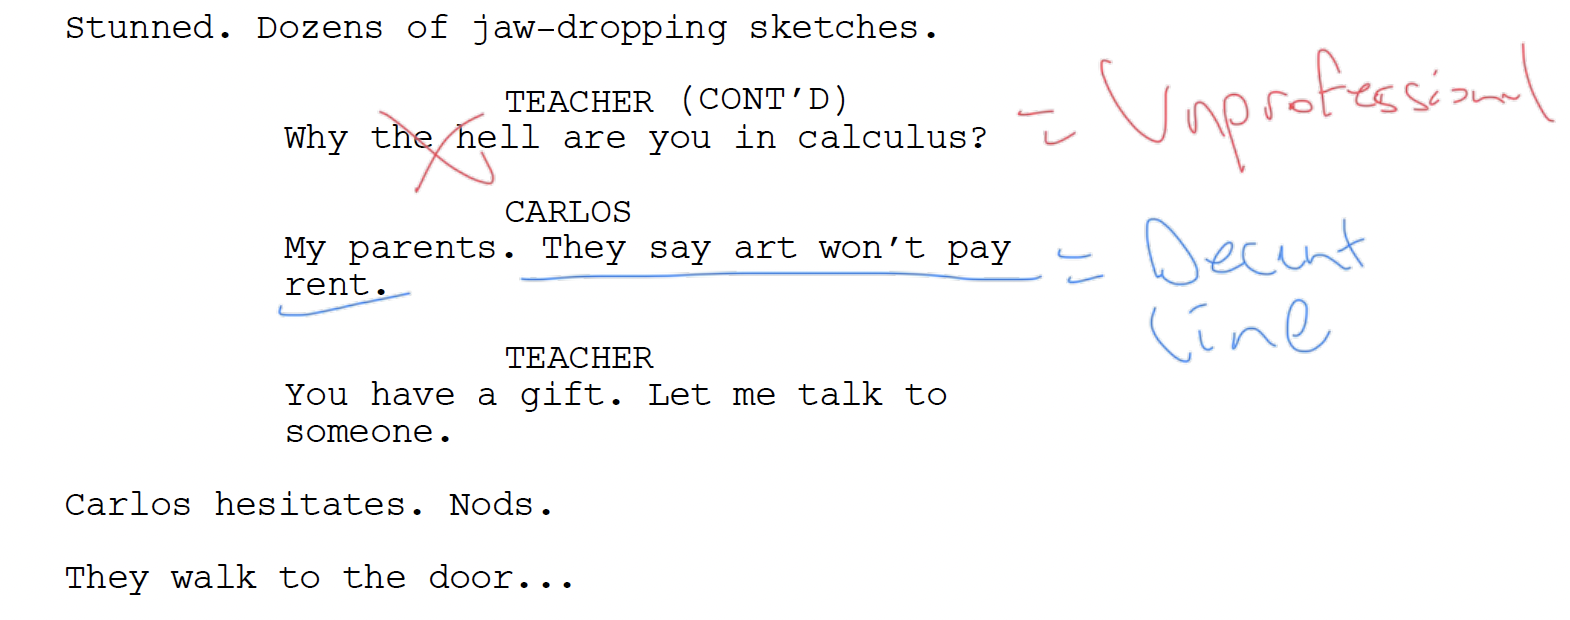
\includegraphics[width=0.8\linewidth]{images/TeacherSwearing.png}
            \caption{A teacher suddenly uses language they never used in the treatment, though Carlos' response is a memorable line}
            \label{fig:a2-teacher}
        \end{figure}
    \begin{description}
        \item[Coherency] was improved a slight bit compared to A1, only having 12 logical breaks rather than 14, giving a $-2/10$ score. However, some of the breaks from logic here are particularly odd. A high school teacher who didn't swear in the treatment suddenly does (Figure 8), Carlos still acts too "nice", the script implies Dahlia and Carlos already knew each other before meeting, there's conversations happening in different places to in the treatment, the hospital doesn't seem to have doctors, and not only is there once again a strange added voiceover, there's even some sort of omniscient narrator added simply dubbed "Night" (Figure 9).
        \begin{figure}[!hbt]
            \centering
            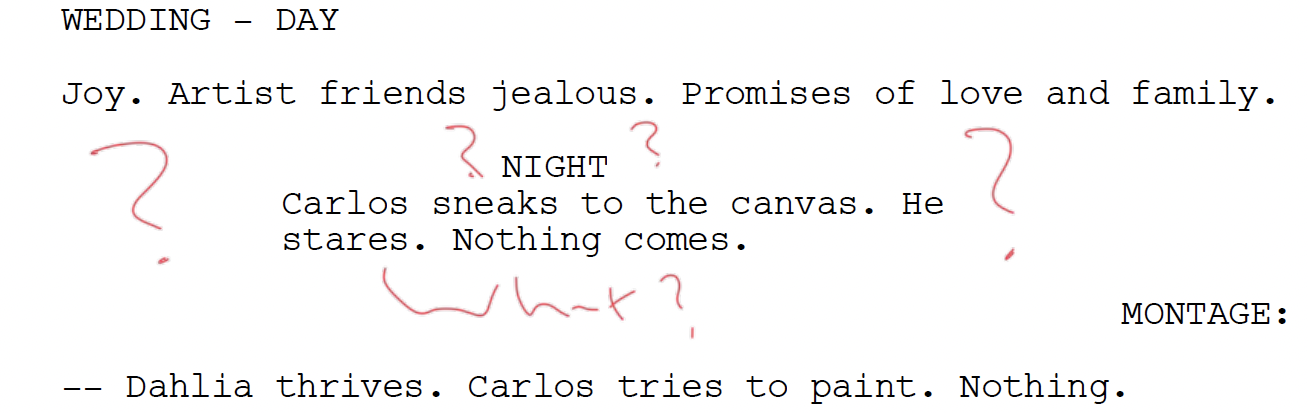
\includegraphics[width=0.8\linewidth]{images/NightNarrator.png}
            \caption{A.I. can still struggle with NER, and believe a time of day may be a character or narrator}
            \label{fig:a2-night-narrator}
        \end{figure}
        \item[Pacing] is once again a big problem with this script overusing montages and rushing past scenes far too fast. In fact, many scenes are rushed enough to become classified as coherency errors rather than just pacing errors. However, it was also still an improvement over Trial 1, having $6$ major pacing infractions as opposed to 9.
        \begin{figure}[!hbt]
            \centering
            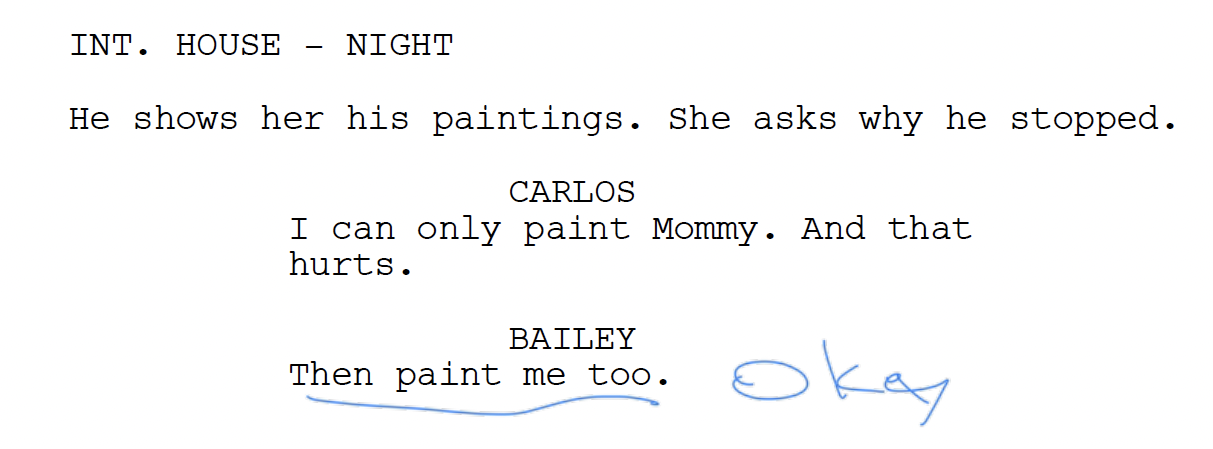
\includegraphics[width=0.8\linewidth]{images/GoodMoment.png}
            \caption{A rare moment of a memorable piece of dialogue in these scripts}
            \label{fig:a2-dialouge}
        \end{figure}
        \item[Imagery] A2 did not have any memorable images like A1 did, but it did contain two moments of memorable dialogue, including one for the little girl that gives her a moment of direct agency over her father that actually serves the scene quite well (Figure 10). Thus I'll give A2 a $2$ for imagery.
    \end{description}
    \item[S] Short Treatment Script
    \begin{description}
        \item[Coherency] was a bit interesting with this script. In terms of actual hard breaks of logic or character or context, I only really noticed 5, but that may be because the script is so marathon in pacing that it doesn't really even feel like there's a flow to "break" from necessarily. Some context is missing, but the characters somehow fit my original treatment better than they did in the other A.I. trials. I'd say a $5/10$ coherence score is odd, but technically fair.
        \item[Pacing] This script has the pacing problems the worst. As can be spotted in Figure 11, the model chose to space out lines way more than is standard, meaning this script is not only the shortest of the bunch, but is shorter even compared to my original treatment. Everything is rushed through to the point where I stopped counting the breaks from pace at some point. Looking over it again, I'd say every single one of the 16 scenes feels extremely rushed, so I'm going to judge this at a $-6/10$.
        \begin{figure}[!hbt]
            \centering
            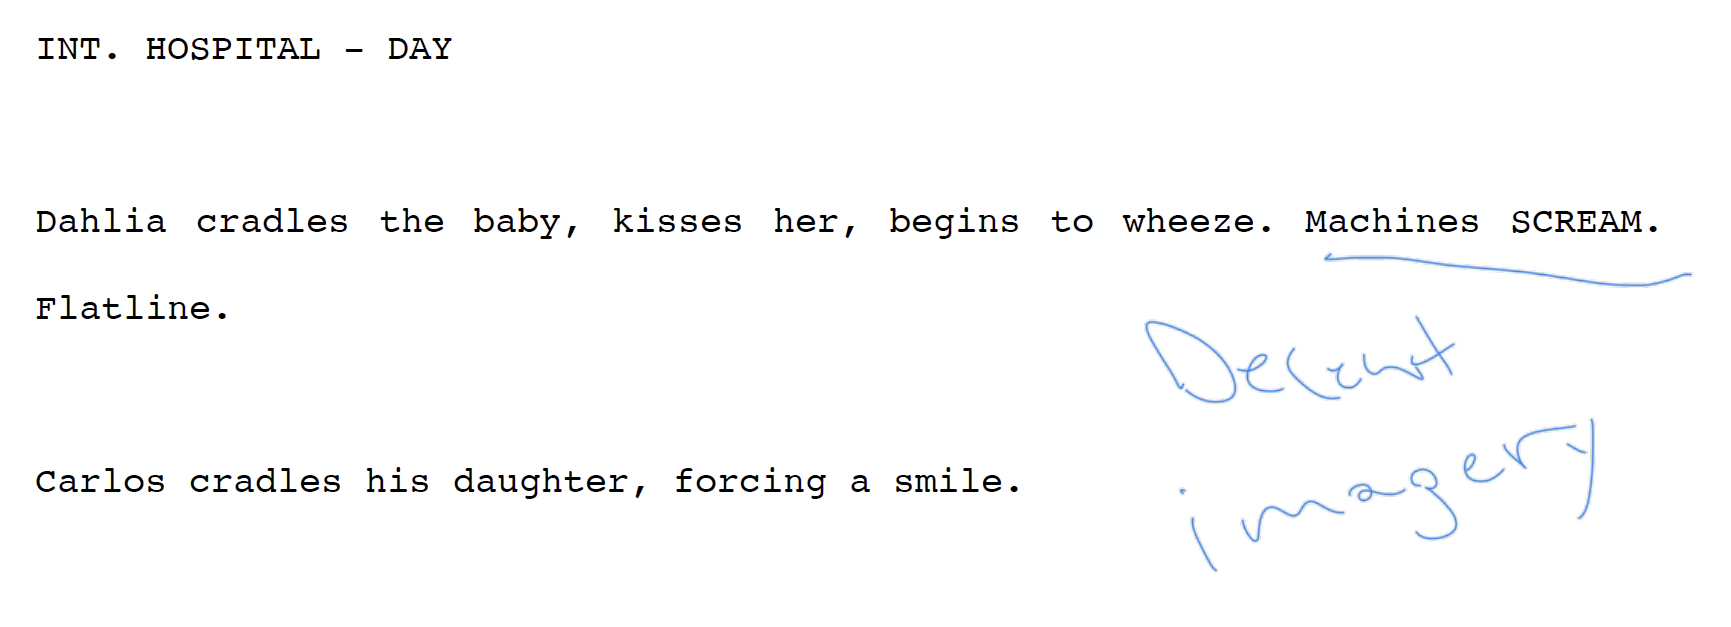
\includegraphics[width=0.8\linewidth]{images/ShortImagery.png}
            \caption{A memorable audiovisual image in an otherwise extremely barebones script}
            \label{fig:s-imagery}
        \end{figure}
        \item[Imagery] This script lacked memorable dialogue entirely, but did have so far the best use of audiovisual imagery in the A.I. scripts, which I show in Figure 11. So another $1$ point for imagery here.
    \end{description}
    \item[H] In terms of judging my own screenplay, I felt it wouldn't be fair to try to present an objective critique of it. I will say that I caught some coherence and pacing issues and feel I could improve the imagery. I annotated my script the same way I did the A.I. ones in the Git Repo. But for an actual measurement I decided to leave that to the ChatGPT model.
\end{description}
\subsection{Critiques}
\begin{description}
    \item[A1] A.I. Trial 1
    \begin{figure}[!hbt]
            \centering
            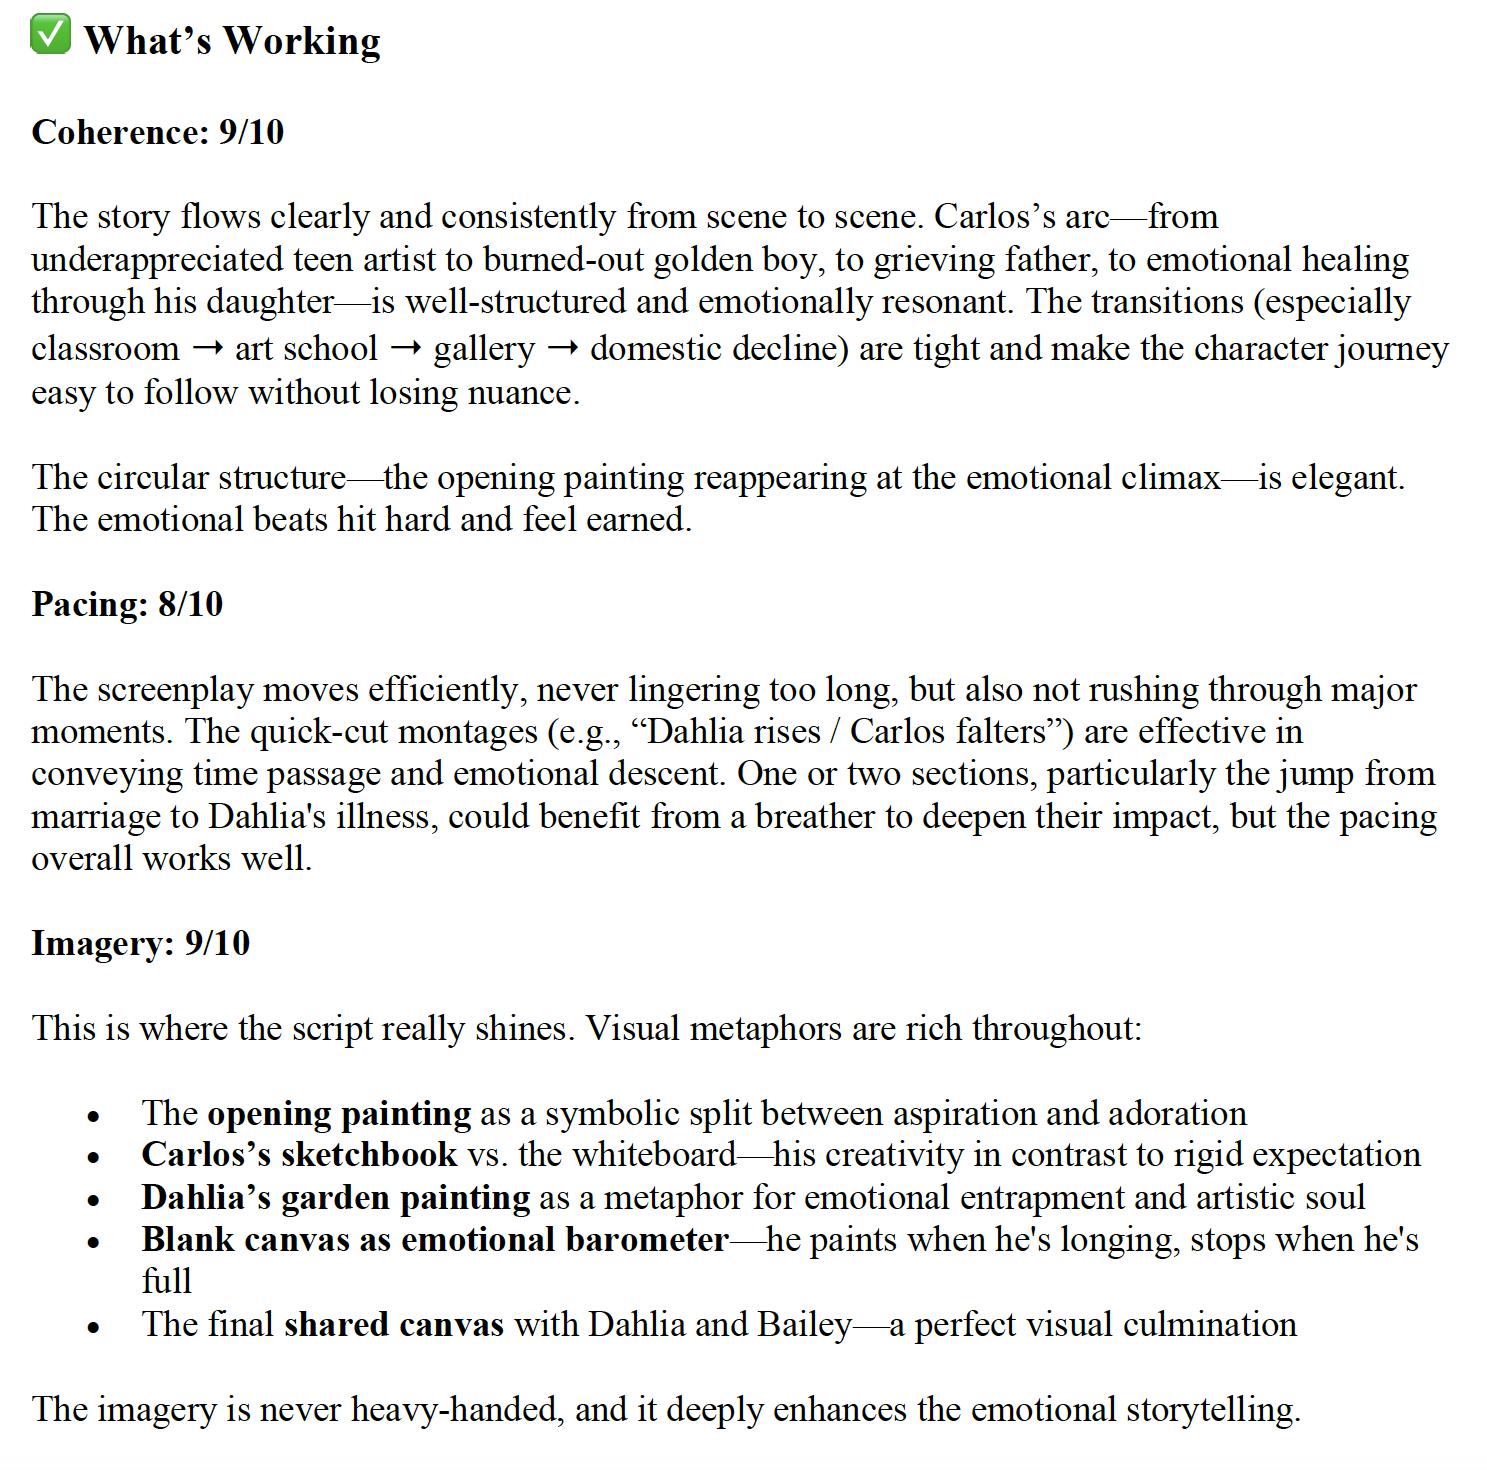
\includegraphics[width=0.5\linewidth]{images/A1Metrics.png}
            \caption{ChatGPT's review of Script A1}
            \label{fig:a1-metrics}
    \end{figure}
    \begin{description}
        \item[Accuracy] in these metrics is very flawed. The LM understands the fundamental idea of a character arc for coherence and not wanting to drag pace, but not the idea of logical flow to such things. The existence of Carlos' character arc alone does not indicate coherence, nor does the existence of quick montages indicate an engaging pace. The LM is extrapolating a deeper meaning to the arc that wasn't conveyed in the script, as well as misreading a rushed summary as an effective montage. As well, all five points of imagery noted are points of symbolism, not descriptive imagery, which brings it up to 7 inaccuracies with the script being judged, for an accuracy score of $3/10$.
        \begin{figure}[!hbt]
            \centering
            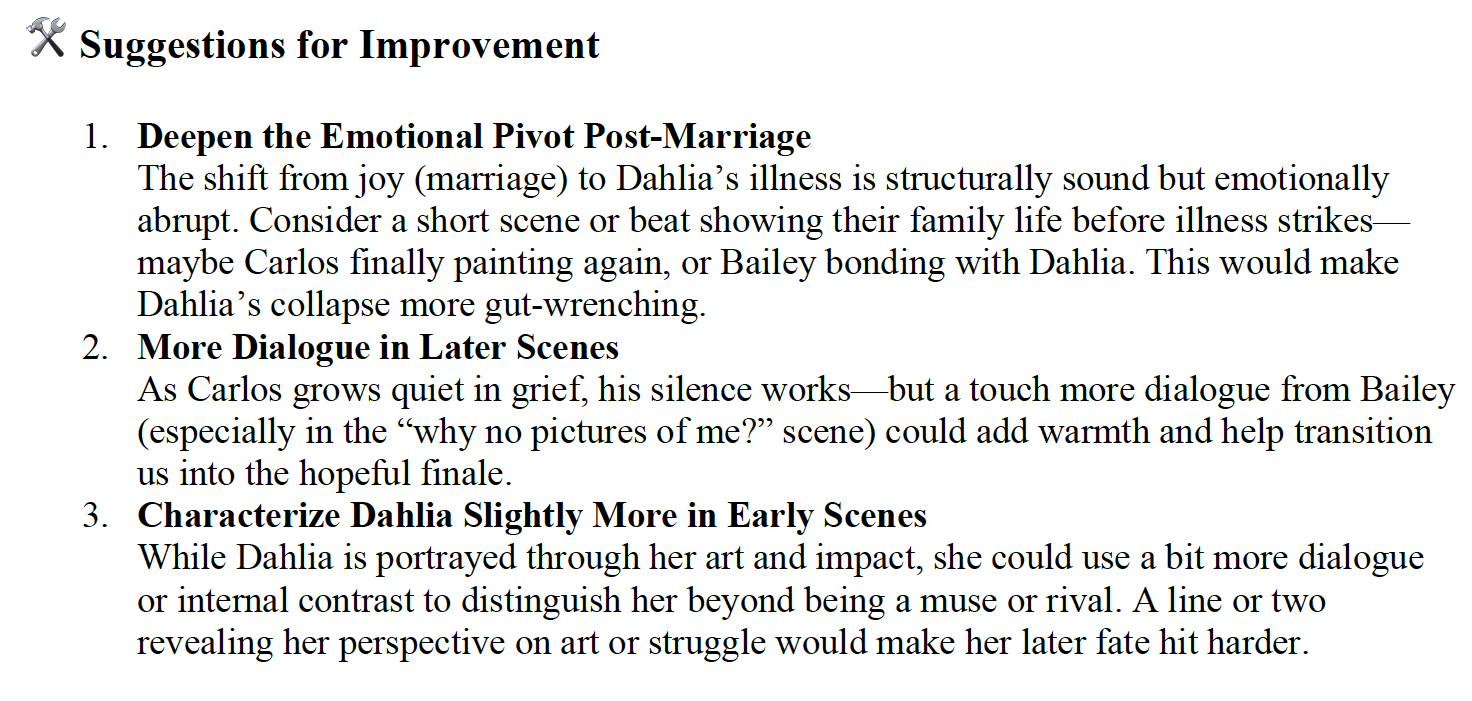
\includegraphics[width=0.8\linewidth]{images/A1Improvements.png}
            \caption{ChatGPT's improvements for Script A1}
            \label{fig:a1-improvements}
        \end{figure}
        \item[Constructiveness] unlike all the other metrics I've used so far, was actually considerably successful in these trials. It was the one thing the model consistently did well, give actionable improvements to the script. All three suggestions for this script are good ideas that would not only make the script at hand better, but are ideas that would make my own better as well. That's a solid $3$ points from every suggestion.
    \end{description}
    \item[A2] A.I. Trial 2
    \begin{figure}[!hbt]
            \centering
            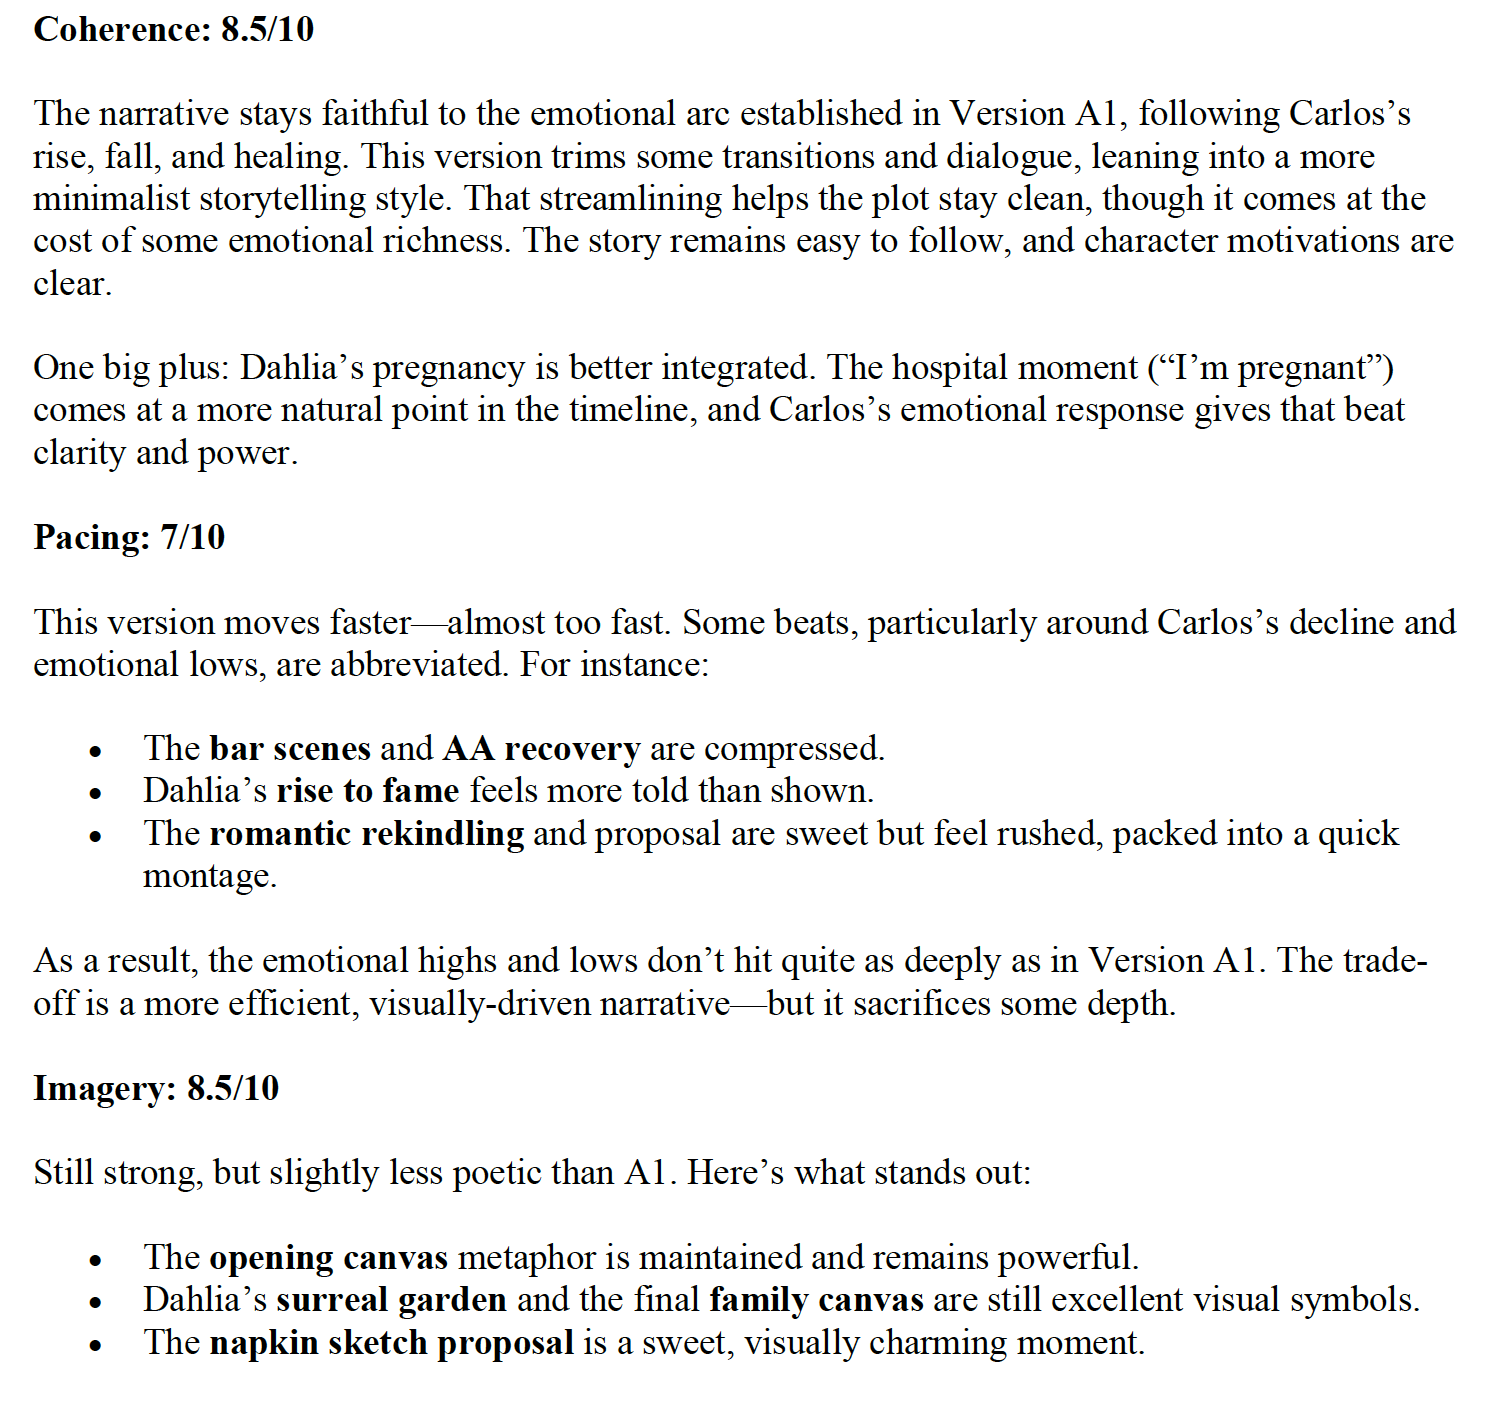
\includegraphics[width=0.5\linewidth]{images/A2Metrics.png}
            \caption{ChatGPT's review of Script A2}
            \label{fig:a2-metrics}
    \end{figure}
    \begin{description}
        \item[Accuracy] is once again an issue. Some breaks in accuracy here include praising the rushed style as "minimalist", claiming the characters have conveyed motivations in this script, and claiming Carlos' response to Dahlia being pregnant was "emotional", when Carlos didn't actually respond to Dahlia being pregnant at all, it was skipped over. Imagery is once again confused for symbolism, outside of the napskin sketch proposal moment, which is an insightful praise to give considering I cut it out of my own script. The pacing faults are actually quite accurate, albeit undercut by not recognizing the same faults in A1. Still, that leaves the accuracy at a $5/10$.
        \begin{figure}[!hbt]
            \centering
            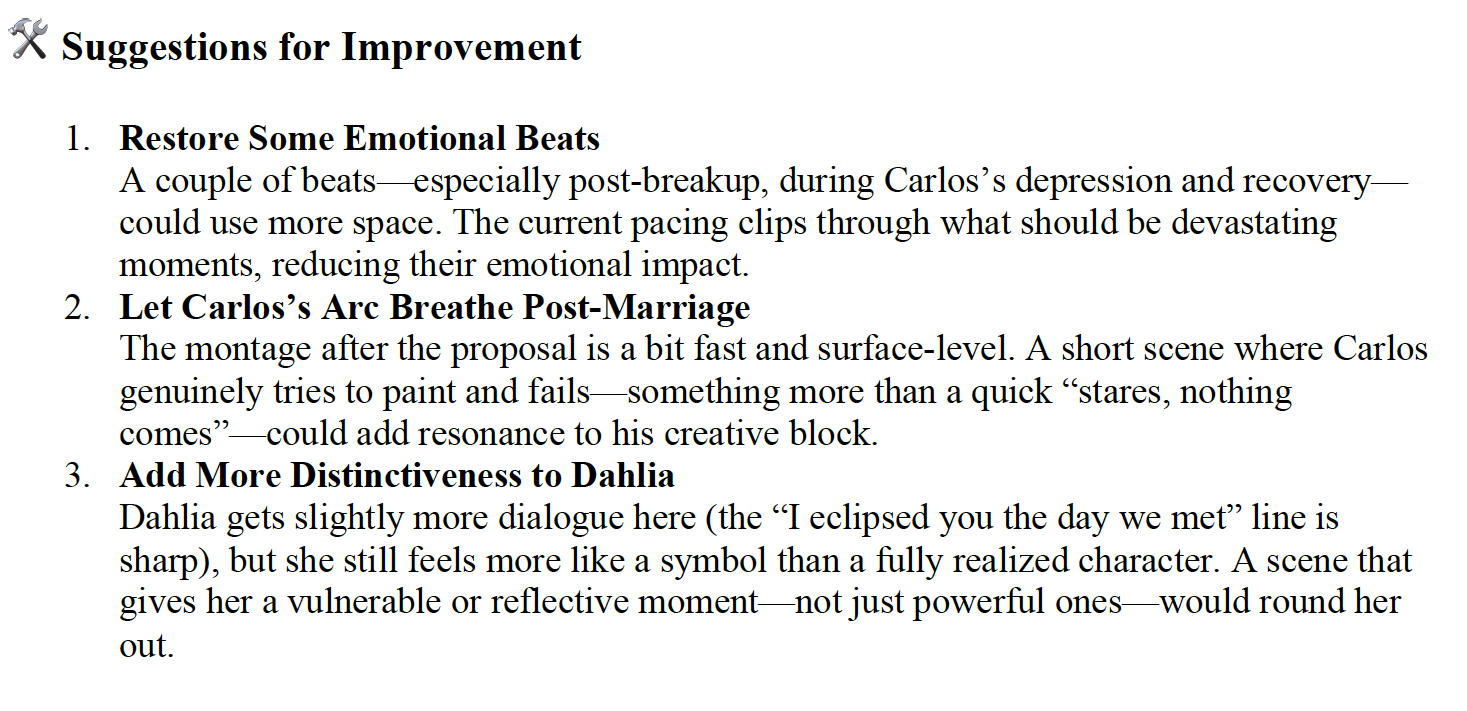
\includegraphics[width=0.8\linewidth]{images/A2Improvements.png}
            \caption{ChatGPT's improvements for Script A2}
            \label{fig:a2-improvements}
        \end{figure}
        \item[Constructiveness] once again was a success. The second two suggestions are ones that my script could benefit from, while the first still finds a room for improvement in the A.I. script being analyzed. Once again, a full $3$ points for every suggestion.
    \end{description}
    \item[S] Short Treatment Script
    \begin{figure}[!hbt]
            \centering
            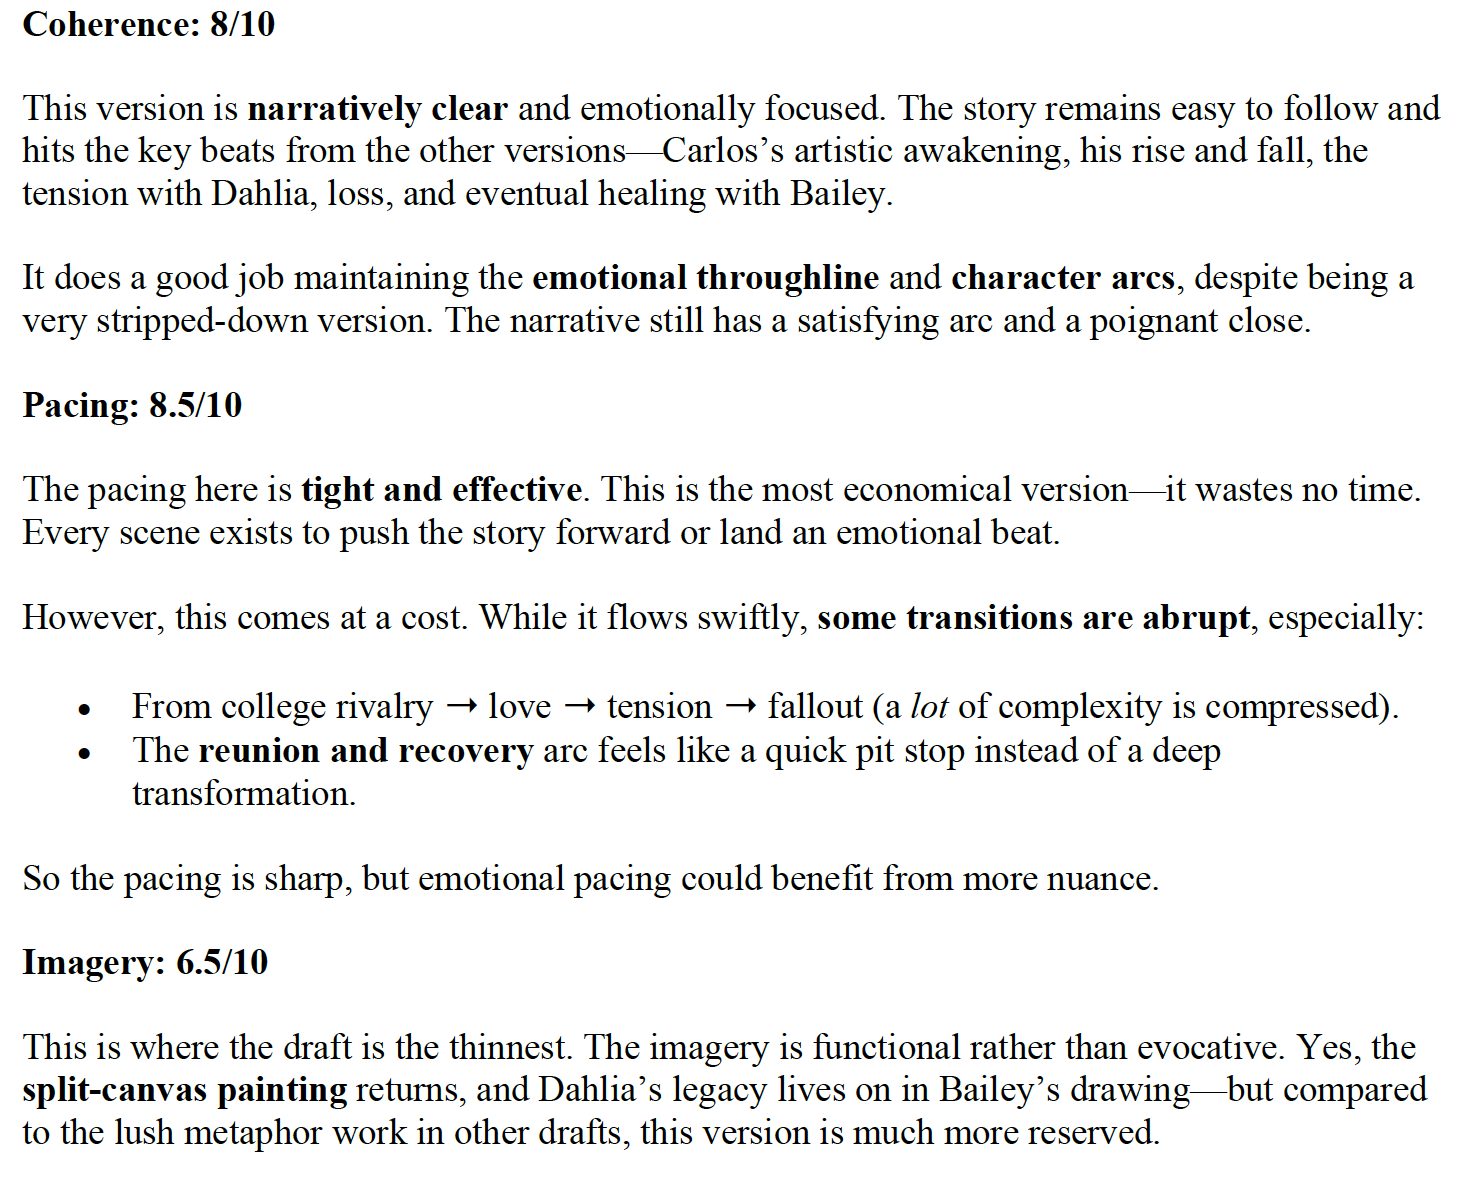
\includegraphics[width=0.5\linewidth]{images/SMetrics.png}
            \caption{ChatGPT's review of Script S}
            \label{fig:s-metrics}
    \end{figure}
    \begin{description}
        \item[Accuracy] is at an all-time low with this review. Emotion was hardly the focus on the S script, there weren't really character arcs, scenes don't land emotional beats or really push the story forwards. Once more, imagery is confused for metaphor and symbolism, rather than descriptive details and setting. The pacing faults, once again, aren't necessarily wrong so much as they are issues the LM should've caught in the other scripts. This reads at around $4/10$ accuracy.
        \begin{figure}[!hbt]
            \centering
            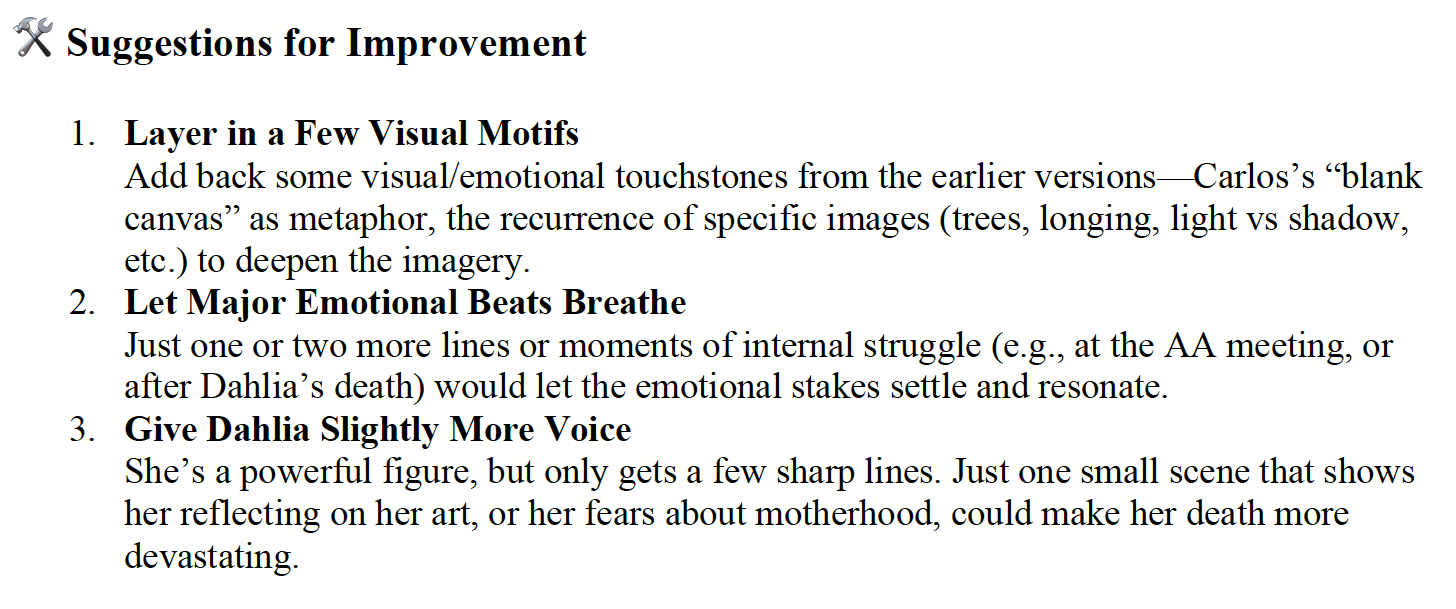
\includegraphics[width=0.8\linewidth]{images/SImprovements.png}
            \caption{ChatGPT's improvements for Script S}
            \label{fig:s-improvements}
        \end{figure}
        \item[Constructiveness] is slightly less well-handled here. Suggestions 2 and 3 are legitimate improvements, while suggestion 1 is spent on simply asking for more metaphors, which doesn't really seem like the solution to the larger problems of the script. $2/3$.
    \end{description}
    \item[H] Human Script
    \begin{figure}[!hbt]
    \centering
    \begin{minipage}{0.2\textwidth}
        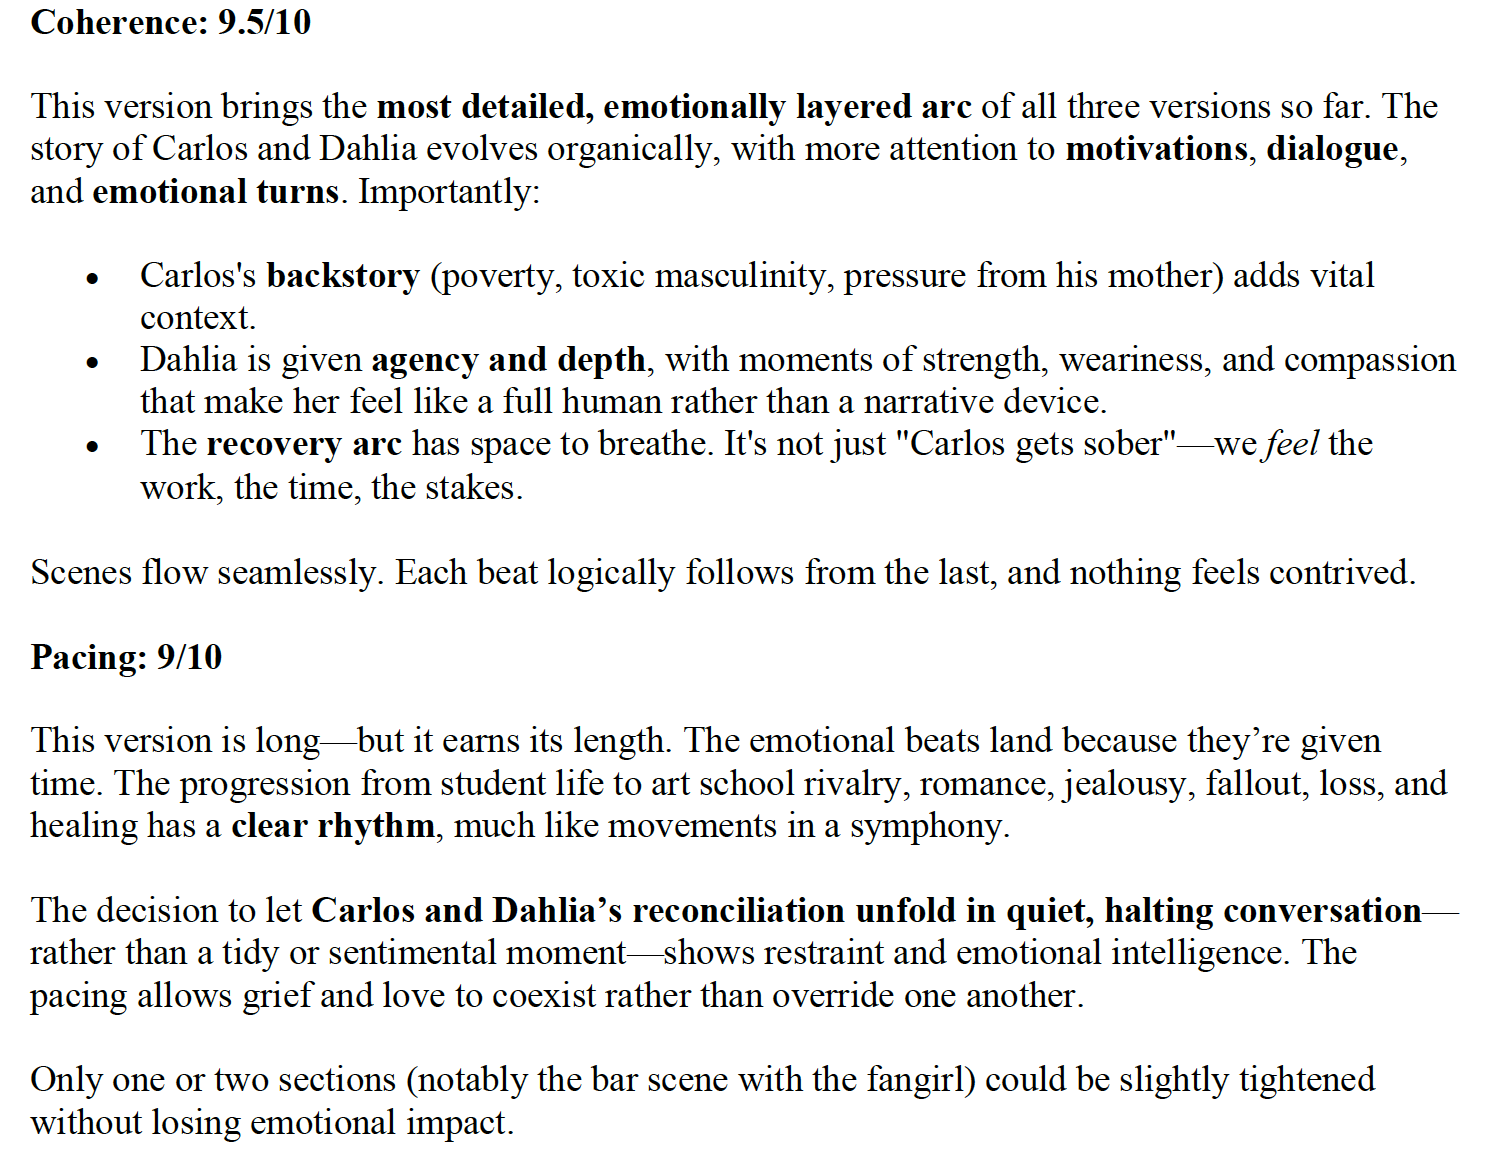
\includegraphics[width=1.0\linewidth]{images/HMetrics1.png}
        \caption{Coherence and Pacing scores on my screenplay}
        \label{fig:h-metrics-1}
    \end{minipage}\hfill
    \begin{minipage}{0.2\textwidth}
        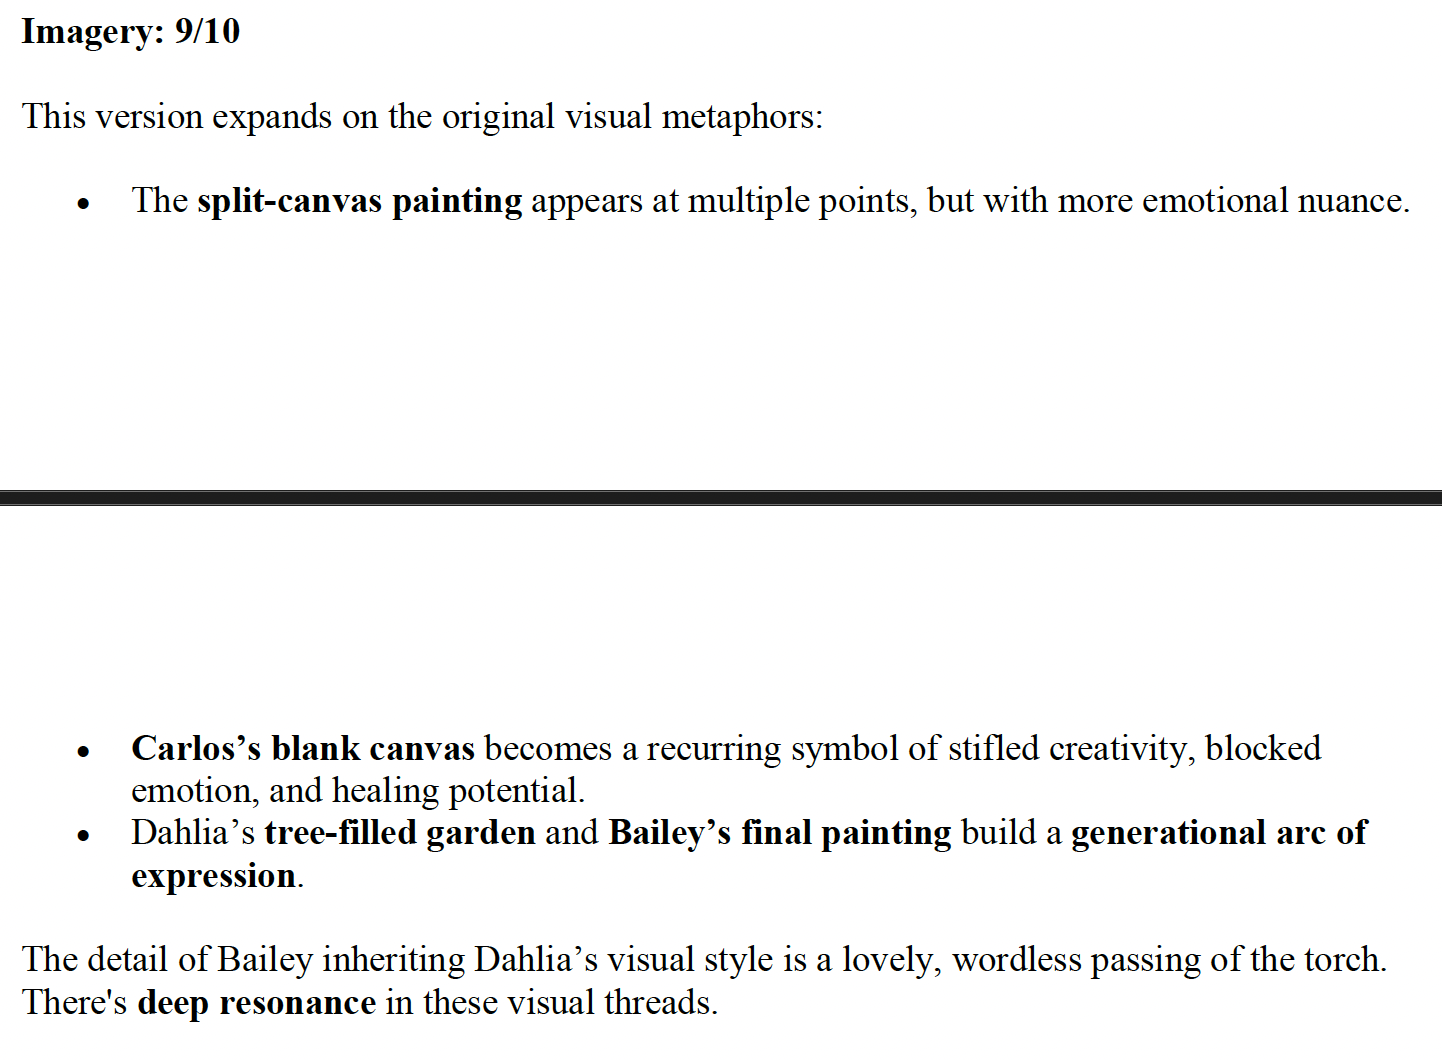
\includegraphics[width=1.0\linewidth]{HMetrics2.png}
        \caption{Imagery score on my screenplay}
        \label{fig:h-metrics2}
    \end{minipage}
\end{figure}
    \begin{description}
        \item[Accuracy] is certainly better when given a human script to judge. That the model understands the point of Carlos' flaws and toxicity is a significant step up from what we've seen so far. However, it could still be more critical. The recovery arc doesn't really have space to breathe, it's jumped over in a timeskip even in my script. And once again, every attempt to explain imagery is once again overly focused on symbolism rather than the visual detail I was looking to judge. $6/10$ accuracy here.
        \begin{figure}[!hbt]
            \centering
            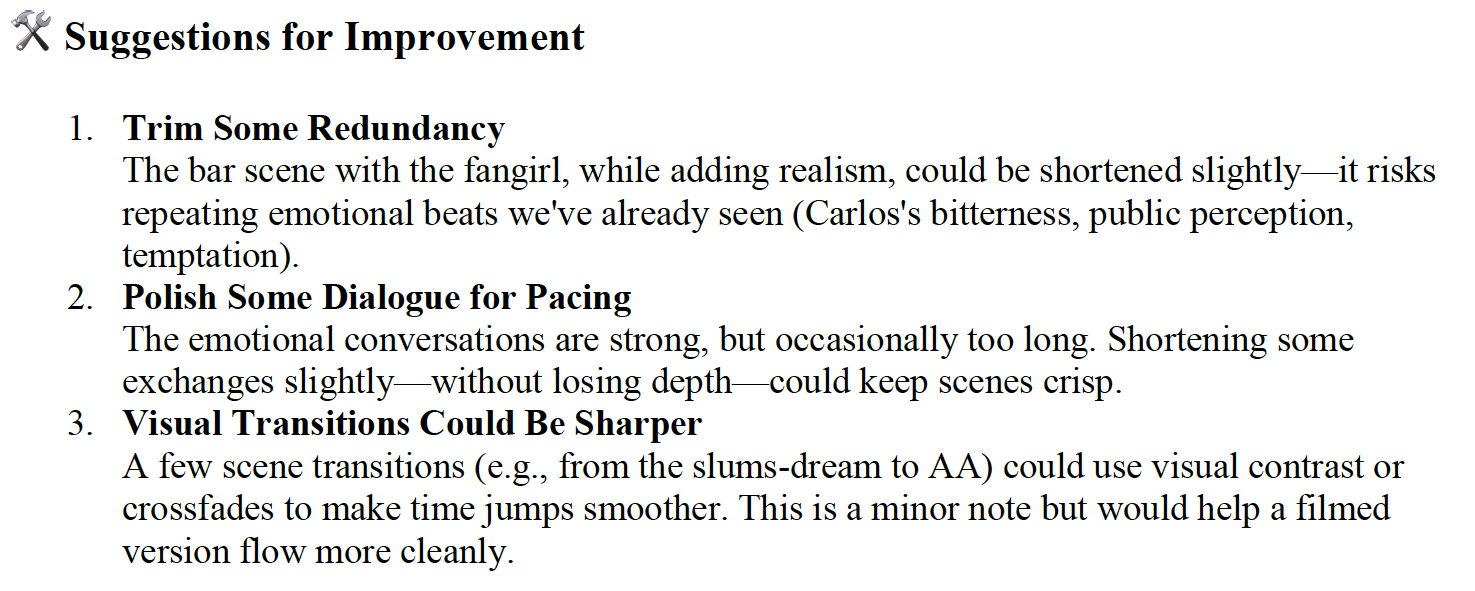
\includegraphics[width=0.8\linewidth]{images/HImprovements.png}
            \caption{ChatGPT's improvements for my screenplay}
            \label{fig:h-improvements}
        \end{figure}
        \item[Constructiveness] is actually considerably weaker here. Many of the suggestions offered the A.I. scripts are more tangible and realistic improvements. These suggestions include a slight redundancy as two of them deal mostly with trimming down overlong dialogue scenes, and the last one is a visual nitpick rather than a deeper issue. Only $1/3$ this time.
    \end{description}
\end{description}

\section{Discussion and Challenges}
\subsection{Insights}
\indent In spite of how far LLMs have come, it's clear in these results that there's still a fundamental lack of understanding of creative or narrative structures and storytelling in them. Given the concerns raised during the WGA strikes, I had expected to find A.I. at least capable of creating something approaching human level. But what I found is that even with detailed instructions, these models won't really generate much beyond what you give them. Once more, I instructed every single model to write at least 20 pages, and the most I ever received back was 6.\\
\indent More telling was how poorly ChatGPT seemed to understand analyzing its own scripts, often finding its own work to be near-perfect in spite of clear, visible flaws. It took viewing a complete human screenplay for the model to show even a rudimentary understanding of the intended arcs and ideas of the story it had been given to begin with. The fact that it was able to reach that point, and consistently hinted towards it when giving suggestions for improvement, is proof that this potential does lie in these models, there's just something holding them back.
\subsection{Threats to Validity and Improvements}
\indent Some limitations and potential confounding variables in this study included the use of specialized ChatGPT models such as "Creative Writing Coach" and "Write For Me". Perhaps a vanilla ChatGPT session would've granted different results, or a non-ChatGPT-based model. The model never being exposed to the fully fleshed-out screenplay until critiques could also be a concern, as being trained on the final human output could potentially benefit generation.\\
Testing entirely on one already defined story idea may also have been a limiting factor. Had I taken the idea from brainstorming with ChatGPT, it may have been able to develop the idea better. In the future it would also be wise to find ways to force the model to adhere to page counts and reach the same length of screenplay as the human script, in order to have space to generate more than a basic rewording of the treatment.

\section{Conclusion}
While this study is hardly conclusive, it does add to the increasing litany of research showing that A.I. has harsher limits in these creative endeavors than some might've believed. At no point in the process, other than suggestions for improvement during critique, did these A.I. models ever create anything approaching human quality. Ethically, that may even be a good thing, keeping these models relegated to editors and aids to professional writers, rather than competition. Even so, there is a clear potential buried underneath for these models to improve understanding of creative concepts. How that will be used is yet to be seen.

\bibliographystyle{ACM-Reference-Format}
\bibliography{references.bib}
\end{document}
